\documentclass[11pt,a4paper]{article}

\usepackage[T1]{fontenc}
\usepackage[utf8]{inputenc}
\usepackage{lmodern}
\usepackage{microtype}
\usepackage[a4paper,margin=25mm]{geometry}
\usepackage{amsmath,amssymb,amsthm,mathtools}
\usepackage{bm}
\usepackage{booktabs}
\usepackage{array}
\usepackage{enumitem}
\usepackage{xcolor}
\usepackage{hyperref}
\usepackage{setspace}
\usepackage{fancyhdr}
\usepackage{tikz}
\usetikzlibrary{arrows.meta,calc,positioning}

\definecolor{navy}{HTML}{17365D}
\definecolor{slate}{HTML}{394B59}
\definecolor{lightblue}{HTML}{EAF1F8}
\definecolor{lightgray}{HTML}{F3F5F7}

\hypersetup{
  colorlinks=true,
  linkcolor=navy,
  citecolor=navy,
  urlcolor=navy,
  pdftitle={Chronometry from Crossed Null Phases},
  pdfsubject={Research note on emergent proper time from null phase relations}
}

\setstretch{1.08}
\setlength{\parindent}{0pt}
\setlength{\parskip}{0.62em}
\setlist[itemize]{leftmargin=1.55em,itemsep=0.25em,topsep=0.25em}
\setlist[enumerate]{leftmargin=1.75em,itemsep=0.25em,topsep=0.25em}

\pagestyle{fancy}
\fancyhf{}
\fancyhead[L]{\small\color{slate}Chronometry from Crossed Null Phases}
\fancyhead[R]{\small\color{slate}Working paper v0.1}
\fancyfoot[C]{\thepage}
\renewcommand{\headrulewidth}{0.3pt}

\newtheorem{definition}{Definition}[section]
\newtheorem{theorem}[definition]{Theorem}
\newtheorem{proposition}[definition]{Proposition}
\newtheorem{corollary}[definition]{Corollary}
\newtheorem{remark}[definition]{Remark}
\newtheorem{conjecture}[definition]{Conjecture}

\newcommand{\M}{\mathcal{M}}
\newcommand{\dd}{\mathrm{d}}
\newcommand{\Lie}{\mathcal{L}}
\newcommand{\R}{\mathbb{R}}
\newcommand{\Sph}{\mathbb{S}}
\newcommand{\Xcross}{X}
\newcommand{\Ccross}{C}
\newcommand{\ThetaClock}{\Theta}
\newcommand{\Order}{\prec}
\newcommand{\Lag}{\mathcal{L}}
\newcommand{\UV}{\mathrm{UV}}
\newcommand{\IR}{\mathrm{IR}}
\newcommand{\sgn}{\operatorname{sgn}}

\begin{document}
\pagenumbering{gobble}

\begin{titlepage}
\thispagestyle{empty}
\vspace*{18mm}

{\color{navy}\rule{\textwidth}{1.2pt}}
\vspace{8mm}

{\fontsize{24}{29}\selectfont\bfseries\color{navy} Chronometry from Crossed Null Phases\par}
\vspace{4mm}
{\Large A conformal-completion theorem and a dynamical scale-locking mechanism\par}

\vspace{12mm}

\begin{center}
\begin{minipage}{0.88\textwidth}
\colorbox{lightblue}{\parbox{0.94\textwidth}{
\textbf{Central proposal.} Causal order and null propagation are taken as primitive. Two crossed, physically normalized null phases select a timelike clock direction and a spacelike ruler direction. An interaction-generated mass gap fixes their common scale. Proper duration is then reconstructed as phase count, rather than inserted as a primitive clock parameter.
}}
\end{minipage}
\end{center}

\vfill

\begin{tabular}{@{}ll@{}}
Document status: & Exploratory research note; not peer reviewed \\
Version: & 0.1 \\
Date: & 13 August 2026 \\
Scope: & Exact kinematics, effective dynamical model, falsifiability criteria
\end{tabular}

\vspace{10mm}
{\color{navy}\rule{\textwidth}{1.2pt}}
\end{titlepage}
\pagenumbering{roman}

\begin{abstract}
A single null direction supplies causal orientation but no proper-time standard. This note studies whether a pair of null degrees of freedom can supply one. Let $(\M,[g])$ be a time-oriented conformal Lorentzian manifold and let $\phi_\pm:\M\rightarrow \Sph^1$ be compact phases whose gradients are future-directed, null, and nonparallel. On every region where
\[
\Ccross=-\frac12 g^{ab}\nabla_a\phi_+\nabla_b\phi_->0,
\]
we define
\[
h_{ab}=\Ccross g_{ab},\qquad
T=\frac{\phi_++\phi_-}{2},\qquad
R=\frac{\phi_+-\phi_-}{2}.
\]
We prove that $h_{ab}$ is invariant under Weyl rescaling and is the unique representative of the conformal class for which $\dd T$ and $\dd R$ are orthogonal unit timelike and spacelike covectors. Reciprocal rescaling of the two null gradients acts exactly as a Lorentz boost on $(\dd T,\dd R)$, while their common rescaling changes the chronometric scale. Thus the ratio of null normalizations is rapidity and their geometric mean is clock calibration.

To make that calibration dynamical, we propose a Weyl-covariant effective model in which a crossed-phase invariant $\Ccross$ is locked to an order parameter $\Sigma$ generated by dimensional transmutation in an interacting massless sector. Its homogeneous vacuum satisfies $\Ccross=\Sigma=\Lambda^2$, so the same interaction that generates a mass gap also fixes the phase clock. The Gross--Neveu mechanism provides an explicit lower-dimensional proof of principle: interacting left- and right-moving massless modes generate a timelike mass shell, fixing the product of their light-cone momenta while leaving the ratio as ordinary rapidity. We formulate a clock-universality criterion, extend the construction to many-ray radiation states, identify degeneracies and global obstructions, and distinguish the exact results from the conjectural physics.
\end{abstract}

\tableofcontents
\clearpage
\pagenumbering{arabic}

\section{Question and answer in one page}

The question is not whether one can write coordinates in which a photon has constant position. That is easy and does not create an observer. The sharper question is:

\begin{quote}
Can a theory begin with causal/null relations but no primitive duration scale, and dynamically construct both a timelike direction and a reproducible clock rate?
\end{quote}

The proposed answer has four layers:

\begin{enumerate}
  \item \textbf{Causal layer.} Null incidence determines which events can influence which. This fixes conformal causal geometry but not lengths or durations.
  \item \textbf{Pairing layer.} Two nonparallel null phases define a timelike sum and a spacelike difference.
  \item \textbf{Scale layer.} An interaction-generated mass gap fixes the product of their null frequencies, resolving the missing Weyl scale.
  \item \textbf{Readout layer.} A relative quantum phase or another periodic observable counts the resulting proper duration.
\end{enumerate}

The resulting slogan is
\[
\boxed{
\text{causal order is primitive; chronometric duration is dynamically calibrated.}
}
\]

This is more precise than saying simply that ``time emerges.'' Ordering is already present. What emerges is a unit timelike flow and the conversion of change into reproducible duration.

\section{Relation to established work}

The ingredients have substantial ancestry, so any novelty claim must be narrow.

\begin{itemize}
  \item Causal order determines the conformal metric under standard causality assumptions; an additional scale or volume structure is required to recover a full metric \cite{EPS1972,HKM1976,Malament1977,Braun2025}.
  \item Double-null geometry routinely uses two optical functions with null gradients. Their cross-normalization is encoded in a null lapse. The algebra below is compatible with that formalism, but gives the cross-normalization an explicitly chronometric interpretation \cite{Gourgoulhon2005,Czimek2022}.
  \item Two cross-flowing null-dust streams can be represented as an anisotropic fluid with a preferred internal time, unlike one null stream \cite{Horvath2006,Kovacs2006}.
  \item In Weyl/EPS geometry, a clock protocol can select a representative of a conformal class \cite{Fatibene2022}.
  \item Thermal time derives a state-dependent time flow from a state on an observable algebra \cite{ConnesRovelli1994}.
  \item Dimensional transmutation and radiative breaking of scale symmetry can generate a physical mass scale from classically dimensionless couplings \cite{ColemanWeinberg1973,GrossNeveu1974,Oda2020}.
\end{itemize}

The candidate contribution of this note is the \emph{combined construction}: compact crossed null phases give an exact conformal completion whose sum and difference are already unit clock and ruler covectors; a separate interaction-generated order parameter locks the remaining scale; and a spectral factorization criterion states when different physical clocks recover one and the same chronometric metric.

\section{Primitive data}

Work on a four-dimensional, time-oriented Lorentzian manifold $\M$ with signature $(-,+,+,+)$. Initially assume only a conformal class
\[
[g]=\{\Omega^2 g\,|\,\Omega:\M\to\R_{>0}\}.
\]
Conformal representatives agree on null cones and causal order but not on proper duration.

Let
\[
\phi_+,\phi_-:\M\rightarrow \Sph^1
\]
be two compact phase fields. Locally they may be unwrapped to real functions, but globally only their differentials and winding data need be single-valued. Define
\[
k_a=\nabla_a\phi_+,
\qquad
\ell_a=\nabla_a\phi_-.
\]
Assume, on an open region $\mathcal U\subset\M$,
\begin{align}
 g^{ab}k_ak_b&=0,\\
 g^{ab}\ell_a\ell_b&=0,\\
 \Ccross:=-\frac12g^{ab}k_a\ell_b&>0.
\end{align}
The final inequality says that the two future null covectors are not parallel. The scalar $\Ccross$ has inverse-length-squared dimensions when the phases are dimensionless.

\begin{remark}[Why phases rather than affine null parameters]
An affine parameter on a null ray is arbitrary under $\lambda\mapsto a\lambda+b$. A physical compact phase carries a distinguished cycle $2\pi$. This does not yet provide seconds, but it converts otherwise arbitrary null labels into countable physical cycles. The remaining physical question is what selects their frequency scale.
\end{remark}

\section{The crossed-null chronometric completion}

Define the average and difference phases
\begin{equation}
T=\frac{\phi_++\phi_-}{2},
\qquad
R=\frac{\phi_+-\phi_-}{2},
\label{eq:TRdef}
\end{equation}
and define the dimensionless chronometric metric
\begin{equation}
\boxed{h_{ab}=\Ccross g_{ab}.}
\label{eq:hdef}
\end{equation}
Here $h$ measures intervals in phase cycles. A conventional metric with units of length squared is obtained only after choosing a unit convention, for example $g^{\rm phys}_{ab}=h_{ab}/\Lambda_0^2$ for a declared reference frequency $\Lambda_0$.

\begin{theorem}[Crossed-null completion]
On every region where the assumptions above hold:
\begin{enumerate}
  \item $h_{ab}$ is independent of the representative $g\in[g]$;
  \item $\dd T$ is unit timelike with respect to $h$;
  \item $\dd R$ is unit spacelike with respect to $h$;
  \item $\dd T$ and $\dd R$ are $h$-orthogonal;
  \item $h$ is the unique conformal representative for which $\dd T$ has unit timelike norm.
\end{enumerate}
\end{theorem}

\begin{proof}
Under a Weyl transformation $g_{ab}\mapsto\widetilde g_{ab}=\Omega^2g_{ab}$,
\[
\widetilde g^{ab}=\Omega^{-2}g^{ab},
\qquad
\widetilde{\Ccross}=\Omega^{-2}\Ccross.
\]
Hence
\[
\widetilde h_{ab}=\widetilde{\Ccross}\,\widetilde g_{ab}
=(\Omega^{-2}\Ccross)(\Omega^2g_{ab})=h_{ab}.
\]
Next,
\[
\nabla_aT=\frac{k_a+\ell_a}{2},
\qquad
\nabla_aR=\frac{k_a-\ell_a}{2}.
\]
Using nullity and $g^{ab}k_a\ell_b=-2\Ccross$ gives
\begin{align}
 g^{ab}\nabla_aT\nabla_bT&=-\Ccross,\\
 g^{ab}\nabla_aR\nabla_bR&=+\Ccross,\\
 g^{ab}\nabla_aT\nabla_bR&=0.
\end{align}
Since $h^{ab}=\Ccross^{-1}g^{ab}$, the required norms are $-1,+1,0$.

For uniqueness, let $\widehat h_{ab}=\omega^2g_{ab}$ be any representative satisfying
\[
\widehat h^{ab}\nabla_aT\nabla_bT=-1.
\]
Then
\[
-1=\omega^{-2}g^{ab}\nabla_aT\nabla_bT
=-\omega^{-2}\Ccross,
\]
so $\omega^2=\Ccross$ and therefore $\widehat h=h$.
\end{proof}

Define
\begin{equation}
U^a=-h^{ab}\nabla_bT,
\qquad
E^a=h^{ab}\nabla_bR.
\label{eq:UE}
\end{equation}
Then
\[
h_{ab}U^aU^b=-1,
\qquad
h_{ab}E^aE^b=1,
\qquad
h_{ab}U^aE^b=0,
\]
and
\[
U^a\nabla_aT=1,
\qquad
U^a\nabla_aR=0.
\]
Thus $T$ increases at unit rate along the integral curves of $U$, while $R$ is constant on those curves. Because $\dd T$ is exact, this basic two-phase construction produces an irrotational, hypersurface-orthogonal clock congruence.

\begin{corollary}[Clock and ruler from null incidence]
The pair $(\phi_+,\phi_-)$ produces, without first choosing a timelike observer,
\[
\boxed{
\text{one unit timelike covector }\dd T
\quad+\quad
\text{one unit spacelike covector }\dd R.
}
\]
Two additional transverse directions are still required for a complete spatial triad.
\end{corollary}

\section{Product, ratio, Weyl scale, and rapidity}

Consider local positive rescalings of the null covectors,
\[
k\mapsto k'=ak,
\qquad
\ell\mapsto\ell'=b\ell,
\qquad a,b>0.
\]
Write
\begin{equation}
\alpha=\frac12\ln(ab),
\qquad
\eta=\frac12\ln\left(\frac{a}{b}\right),
\label{eq:alphaeta}
\end{equation}
so that
\[
a=e^{\alpha+\eta},
\qquad
b=e^{\alpha-\eta}.
\]
The two independent changes have different meanings:

\begin{itemize}
  \item $\alpha$ is a common dilation. It sends $\Ccross\mapsto e^{2\alpha}\Ccross$ and therefore changes the phase-defined clock scale.
  \item $\eta$ is a reciprocal rescaling. It leaves $\Ccross$ and $h$ invariant and acts as a Lorentz boost.
\end{itemize}

For the reciprocal case $a=e^\eta$, $b=e^{-\eta}$,
\begin{align}
\dd T'&=\cosh\eta\,\dd T+\sinh\eta\,\dd R,\\
\dd R'&=\sinh\eta\,\dd T+\cosh\eta\,\dd R.
\end{align}
This is exactly the $1+1$ Lorentz transformation in the plane spanned by the two null directions.

\begin{proposition}[Null-scale decomposition]
The two scalar degrees of freedom contained in independent positive rescalings of a crossed null pair decompose as
\[
\boxed{
\begin{aligned}
\frac12\ln(ab)&=\text{chronometric/Weyl dilation},\\[1mm]
\frac12\ln(a/b)&=\text{Lorentz rapidity}.
\end{aligned}}
\]
\end{proposition}

This corrects a tempting but incorrect target. A Lorentz-invariant theory should not dynamically choose one universal value of $\eta$; that would select a preferred inertial frame. It should generate the common scale $e^\alpha$ or, equivalently, $\Ccross$, while a particular state carries its own rapidity. The centre-of-momentum frame of that state is the frame in which the two null contributions are balanced.

\section{Flat-space standing-wave realization}

Let $c=1$ and take Minkowski coordinates $(t,x,y,z)$. Choose counterpropagating phases
\begin{equation}
\phi_+=\omega_+(t-x),
\qquad
\phi_-=\omega_-(t+x),
\qquad \omega_\pm>0.
\label{eq:flatphases}
\end{equation}
Then
\[
\Ccross=\omega_+\omega_-.
\]
Introduce
\[
\bar\omega=\sqrt{\omega_+\omega_-},
\qquad
\eta=\frac12\ln\left(\frac{\omega_+}{\omega_-}\right).
\]
Equation \eqref{eq:TRdef} becomes
\begin{align}
T&=\bar\omega(\cosh\eta\,t-\sinh\eta\,x),\\
R&=\bar\omega(\sinh\eta\,t-\cosh\eta\,x),
\end{align}
and
\[
h_{ab}=\bar\omega^2\eta_{ab}.
\]
In the internally selected centre-of-momentum frame, $\eta=0$ and
\[
T=\bar\omega t,
\qquad
R=-\bar\omega x.
\]
The geometric mean $\bar\omega$ calibrates both tick spacing and ruler spacing.

The complex superposition factorizes as
\begin{equation}
\boxed{
e^{i\phi_+}+e^{i\phi_-}=2e^{iT}\cos R.
}
\label{eq:standingwave}
\end{equation}
For real waves,
\[
\cos\phi_++\cos\phi_-=2\cos T\cos R.
\]
The average phase is a temporal carrier; the difference phase produces stationary spatial nodes. One pair of null waves therefore contains the algebraic form of both a clock and a ruler.

\begin{figure}[ht]
\centering
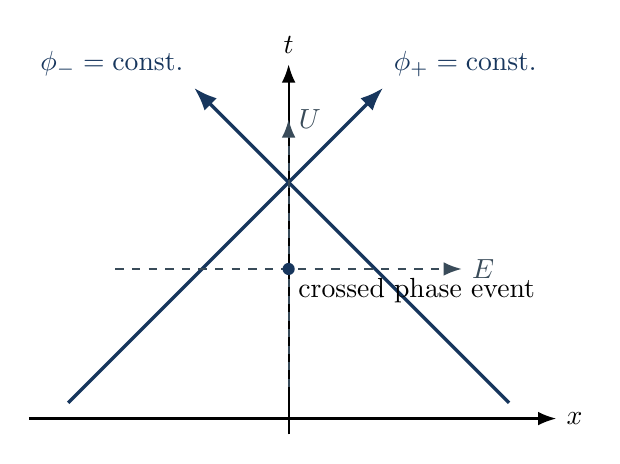
\begin{tikzpicture}[scale=1.0,>=Latex]
  \draw[->,thick] (-3.3,0) -- (3.4,0) node[right] {$x$};
  \draw[->,thick] (0,-0.2) -- (0,4.5) node[above] {$t$};
  \draw[navy,very thick,->] (-2.8,0.2) -- (1.2,4.2) node[above right] {$\phi_+=\mathrm{const.}$};
  \draw[navy,very thick,->] (2.8,0.2) -- (-1.2,4.2) node[above left] {$\phi_-=\mathrm{const.}$};
  \draw[slate,dashed,thick,->] (0,0.4) -- (0,3.8) node[right] {$U$};
  \draw[slate,dashed,thick,->] (-2.2,1.9) -- (2.2,1.9) node[right] {$E$};
  \fill[navy] (0,1.9) circle (2.2pt);
  \node[below right] at (0,1.9) {crossed phase event};
\end{tikzpicture}
\caption{Two crossed null phase families define an internal timelike bisector $U$ and a spacelike difference direction $E$. Their common normalization fixes the chronometric scale; reciprocal normalization changes only rapidity.}
\end{figure}

\section{A dynamical scale-locking mechanism}

The kinematic theorem converts two \emph{physically normalized} phases into a clock. It does not explain why their product should settle at a stable value. We now construct a minimal effective mechanism for that step.

Let
\[
Y_+=g^{ab}\nabla_a\phi_+\nabla_b\phi_+,
\qquad
Y_-=g^{ab}\nabla_a\phi_-\nabla_b\phi_-,
\]
and retain
\[
\Ccross=-\frac12g^{ab}\nabla_a\phi_+\nabla_b\phi_-.
\]
Introduce a positive order parameter $\Sigma$ with mass dimension two and Weyl weight $-2$:
\[
\Sigma\mapsto\Omega^{-2}\Sigma.
\]
The square root $\sigma=\sqrt\Sigma$ is the candidate generated frequency/mass scale.

A schematic effective action is
\begin{equation}
S_{\rm eff}=\int_{\M}\dd^4x\sqrt{-g}\left[
A_+Y_+ + A_-Y_-
-\frac{\kappa}{2}(\Ccross-\Sigma)^2
-V_{\rm DT}(\Sigma)
+\Lag_{\rm kin}(\Sigma)
\right].
\label{eq:Seff}
\end{equation}
The multipliers $A_\pm$ enforce null gradients. With Weyl weight $-2$ for $A_\pm$, the constraint and locking terms are classically Weyl invariant. The term $V_{\rm DT}$ represents the quantum effective potential of an asymptotically free or radiatively broken sector. A convenient local form near its vacuum is
\begin{equation}
V_{\rm DT}(\Sigma)=
\frac{\beta}{4}\Sigma^2
\left(\ln\frac{\Sigma}{\Lambda^2}-\frac12\right)
+\frac{\beta}{8}\Lambda^4,
\qquad \beta>0.
\label{eq:VDT}
\end{equation}
The scale $\Lambda$ is not a classical input parameter. It denotes the renormalization-group invariant generated by dimensional transmutation,
\begin{equation}
\Lambda=\mu\exp\left[-\int^{g(\mu)}\frac{\dd g'}{\beta_g(g')}\right].
\label{eq:RGscale}
\end{equation}
Local Weyl symmetry is therefore broken or anomalous in the effective phase, rather than explicitly broken in the scale-free ultraviolet description.

For homogeneous invariants, define
\begin{equation}
V(\Ccross,\Sigma)=
\frac{\kappa}{2}(\Ccross-\Sigma)^2+V_{\rm DT}(\Sigma).
\label{eq:fullV}
\end{equation}
Its stationary vacuum is
\begin{equation}
\boxed{\Ccross=\Sigma=\Lambda^2.}
\label{eq:vacuum}
\end{equation}
At this point the Hessian in the variables $(\Ccross,\Sigma)$ is
\begin{equation}
H=\begin{pmatrix}
\kappa & -\kappa\\
-\kappa & \kappa+\beta/2
\end{pmatrix}.
\end{equation}
For $\kappa>0$ and $\beta>0$,
\[
H_{11}=\kappa>0,
\qquad
\det H=\frac{\kappa\beta}{2}>0,
\]
so the homogeneous vacuum is a strict local minimum.

At the locked vacuum,
\begin{equation}
\boxed{
h_{ab}=\Lambda^2g_{ab},
\qquad
h^{ab}\nabla_aT\nabla_bT=-1.
}
\label{eq:lockedmetric}
\end{equation}
The dynamically generated mass scale is simultaneously the conformal factor that converts causal geometry into chronometric geometry.

\subsection{What is and is not being fixed}

Equation \eqref{eq:vacuum} fixes the product of the two null frequency scales. It does not fix their ratio. In flat space,
\[
\omega_+\omega_-=\Lambda^2,
\qquad
\frac{\omega_+}{\omega_-}=e^{2\eta}.
\]
The first equation is Lorentz invariant; the second labels a boosted state. In the pair's rest frame, $\eta=0$ and $\omega_+=\omega_-=\Lambda$.

This is the physically acceptable meaning of ``dynamically fixing the relative scale'': the interaction fixes the invariant mass/clock scale and the state itself selects a centre-of-momentum frame. It does not install an aether.

\subsection{A resonance formulation}

The same mechanism can be stated without an order-parameter potential. Suppose two null excitations with momenta $p$ and $q$ form a stable resonance $B$ of dynamically generated mass $M_B$:
\[
p+q\longrightarrow B.
\]
On shell,
\begin{equation}
-(p+q)^2=M_B^2.
\end{equation}
Since $p^2=q^2=0$,
\begin{equation}
\boxed{-2p\cdot q=M_B^2.}
\label{eq:massshelllock}
\end{equation}
The mass shell fixes the invariant product of the two null momenta. Their sum defines the timelike rest direction
\[
U^a=\frac{p^a+q^a}{M_B}.
\]
Thus
\[
\boxed{
\text{mass shell fixes scale; momentum balance fixes frame.}
}
\]

\section{Microscopic proof of principle: massless chiral modes}

The Gross--Neveu family provides an explicit model in which massless left- and right-moving fields interact and generate a mass gap by dimensional transmutation \cite{GrossNeveu1974,Pasnoori2026}. In light-cone variables, a massive on-shell momentum can be written
\begin{equation}
p_+=\frac{m}{\sqrt2}e^\eta,
\qquad
p_-=\frac{m}{\sqrt2}e^{-\eta},
\label{eq:lightconemass}
\end{equation}
so that
\begin{equation}
2p_+p_-=m^2.
\end{equation}
The structure is exact:
\begin{align}
\text{product }p_+p_-&\longleftrightarrow\text{interaction-generated mass scale},\\
\text{ratio }p_+/p_-&\longleftrightarrow\text{rapidity}.
\end{align}
In the massless ultraviolet theory, left and right sectors propagate on separate null directions. Interaction couples them. In the gapped infrared theory, the composite excitation follows a timelike mass shell.

For a convention in which the static $SU(2)$ Gross--Neveu gap is
\[
m=\Lambda_{\UV}e^{-\pi/g},
\]
the dimensionless coupling and ultraviolet cutoff combine into a finite physical scale as the cutoff is removed \cite{Pasnoori2026}. The precise exponent depends on model and coupling conventions; the important point is the nonperturbative generation of a dimensionful gap from dimensionless interaction data.

This is not yet a four-dimensional theory of gravity, but it establishes the required microscopic move:
\[
\boxed{
\text{left-null sector}+\text{right-null sector}+\text{interaction}
\longrightarrow
\text{timelike massive sector}.
}
\]

\section{From a mass gap to an observable clock}

A normalized timelike vector is not by itself a clock readout. A clock requires an observable sequence of distinguishable states. A single stationary quantum state's overall phase is not observable, so use at least two stable levels with energy gap
\[
\Delta E_A=c_A\Lambda,
\]
where $c_A$ is dimensionless. Their relative phase evolves as
\begin{equation}
\dd\Phi_A=\frac{\Delta E_A}{\hbar}\dd\tau_g.
\label{eq:phaseevolution}
\end{equation}
Under $g\mapsto\Omega^2g$, a proper-time element transforms as $\dd\tau_g\mapsto\Omega\dd\tau_g$, while a Weyl-weight $-1$ mass scale transforms as $\Lambda\mapsto\Omega^{-1}\Lambda$. Therefore
\begin{equation}
\boxed{\dd\ThetaClock=\Lambda\,\dd\tau_g}
\label{eq:clockoneformscalar}
\end{equation}
is Weyl invariant, and
\[
\dd\Phi_A=\frac{c_A}{\hbar}\dd\ThetaClock.
\]
After calibration, a count of relative phase cycles is a count of the invariant duration $\ThetaClock$.

In the crossed-phase construction, this invariant is already present geometrically:
\[
\dd\ThetaClock=-\nabla_aT\,\dd x^a
\]
along the congruence $U$. At the locked vacuum $\Lambda^2=\Ccross$, it agrees with \eqref{eq:clockoneformscalar}.

\section{Clock universality as a rank-one spectral condition}

A viable emergent metric must be recovered by every good clock, not just by one specially chosen oscillator.

\begin{theorem}[Local clock universality]
Let $\{\Delta E_A(x)\}$ be the transition energies of a family of clock species on a connected region. They define one common chronometric scale if and only if there exists a positive scalar $\sigma(x)$ and constants $c_A>0$ such that
\begin{equation}
\Delta E_A(x)=c_A\sigma(x)
\label{eq:factorization}
\end{equation}
for every $A$.
Equivalently,
\begin{equation}
\dd\ln\left(\frac{\Delta E_A}{\Delta E_B}\right)=0
\label{eq:ratiocondition}
\end{equation}
for every pair of clock species $A,B$.
\end{theorem}

\begin{proof}
If \eqref{eq:factorization} holds, each clock phase satisfies
\[
\dd\Phi_A=\frac{c_A}{\hbar}\sigma\,\dd\tau_g,
\]
so all clocks differ only by fixed calibration constants and measure the same invariant duration $\dd\ThetaClock=\sigma\dd\tau_g$.

Conversely, if all clocks measure one local duration up to constant calibration, then $\dd\Phi_A/c_A$ is common. Comparing with \eqref{eq:phaseevolution} implies $\Delta E_A/c_A=\sigma(x)$ for one common scalar. Equation \eqref{eq:ratiocondition} is the differential form of the same statement.
\end{proof}

This is a rank-one condition on the spectrum: spacetime dependence may enter all clock gaps only through one common scale. If dimensionless ratios vary, there is no unique chronometric metric. Such variation would appear operationally as differential clock drift and would constitute an equivalence-principle violation rather than merely a change of units.

\section{Scaling up: many photons and the electromagnetic field}

\subsection{Finite collections of null momenta}

For future-directed photon momenta
\[
p_i^a=E_i(1,\widehat{\bm n}_i),
\]
the total momentum is
\[
P^a=\sum_i p_i^a.
\]
Its invariant mass is
\begin{equation}
M^2=-P^2
=2\sum_{i<j}E_iE_j\left(1-\widehat{\bm n}_i\cdot\widehat{\bm n}_j\right).
\label{eq:Nphotonmass}
\end{equation}
All terms are nonnegative. The total remains null only when every occupied direction is parallel. Any genuinely angular distribution has timelike total momentum and therefore a collective rest direction
\[
U^a=\frac{P^a}{M}.
\]
The geometric fact is simple: the future light cone is convex, and a nondegenerate positive mixture of points on its boundary lies in its timelike interior.

This does not make the constituent photons massive. It makes their relation carry invariant mass.

\subsection{Continuum radiation}

For a radiation distribution, replace the finite sum by the stress-energy tensor $T^{ab}$. A local energy frame exists when $T^a{}_b$ has a unique future timelike eigenvector,
\begin{equation}
T^a{}_bU^b=-\rho U^a.
\label{eq:Landau}
\end{equation}
For a pure null beam, $T^{ab}=\rho k^ak^b$, no such timelike rest frame exists. For a non-null electromagnetic field, observers with vanishing Poynting vector do exist, although the principal observer structure need not select one unique worldline without further data \cite{Wylleman2021}.

If $\rho>0$ is the energy density in a distinguished Landau frame, then in four dimensions the state-dependent quantity
\[
\sigma_{\rm rad}=\rho^{1/4}
\]
has the Weyl weight of an inverse length. It yields
\begin{equation}
h^{\rm rad}_{ab}=\rho^{1/2}g_{ab},
\qquad
\vartheta_a=\rho^{1/4}U_a.
\label{eq:radiationclock}
\end{equation}
These are local, state-dependent chronometric objects. They fail where the radiation becomes null, vanishes, or has no unique timelike eigenline.

In a radiation-dominated FLRW model, $\rho\propto a^{-4}$, so
\[
\rho^{1/4}\dd t\propto\frac{\dd t}{a}=\dd\eta_{\rm conformal}.
\]
A radiation-state clock naturally tracks conformal time. This is useful cosmologically but does not by itself provide the persistent, universal scale required of atomic clocks in an empty late-time region.

\subsection{Why source-free Maxwell theory is insufficient}

Vacuum Maxwell theory in four dimensions is linear and conformally invariant. It supplies null propagation, interference, and state-dependent frequencies, but no autonomous mechanism that chooses one universal frequency. A pure electromagnetic realization therefore needs at least one extra ingredient:
\[
\text{nonlinearity, charged matter, a boundary, confinement, gravity, or a quantum anomaly.}
\]
The interaction-generated order parameter in Section 7 is designed to be that ingredient. Literal free photons alone do not complete the proposal.

\subsection{Why ``all photons in the universe'' is not one global vector}

In generic curved spacetime, momenta at different events belong to different tangent spaces and cannot be canonically summed. A cosmological construction should therefore be local: use a distribution function $f(x,p)$ or $T^{ab}(x)$ to define $U^a(x)$ and a local scale. A global cosmic time exists only when the resulting congruence satisfies appropriate integrability conditions. In particular, nonzero vorticity can obstruct a foliation by global simultaneity slices even though local clock directions remain meaningful.

\section{What has emerged, exactly?}

The construction separates several notions often collapsed into the word ``time.''

\begin{center}
\begin{tabular}{>{\raggedright\arraybackslash}p{0.28\textwidth} >{\raggedright\arraybackslash}p{0.29\textwidth} >{\raggedright\arraybackslash}p{0.31\textwidth}}
\toprule
Structure & Status in the proposal & Source \\
\midrule
Causal before/after & Primitive & Null incidence / causal order \\
Local time direction & Derived kinematically & Sum of crossed null covectors \\
Spatial ruler direction & Derived kinematically & Difference of crossed null covectors \\
Duration scale & Derived dynamically & Mass gap / order parameter \\
Tick sequence & Derived operationally & Relative phase of stable levels \\
Global time coordinate & Not guaranteed & Requires integrability and topology \\
Arrow of time & Not derived here & Requires entropy production or asymmetric boundary data \\
\bottomrule
\end{tabular}
\end{center}

So the strongest defensible claim is not that every aspect of time appears from nothing. It is
\[
\boxed{
\text{metric duration can arise as a collective calibration of more primitive causal relations.}
}
\]

\section{Failure modes and consistency conditions}

A serious theory must confront the following points.

\subsection{Degeneracy at parallelism}

When the two null gradients become parallel or one vanishes,
\[
\Ccross\rightarrow0,
\]
and $h_{ab}$ degenerates. A universal theory needs an atlas of overlapping phase pairs, a many-ray construction, or a persistent condensate that prevents loss of rank.

\subsection{Caustics}

Optical phases generically form caustics. The gradients can remain locally defined while a single global phase chart fails. Chronometry must be patched across such regions using invariant phase differences or a network description.

\subsection{Topology}

Because $\phi_\pm$ are circle-valued, $T$ need not be a globally single-valued real function. The one-form $\dd T$ may be closed but not exact globally. Nontrivial periods can encode winding or synchronization holonomy.

\subsection{Universality}

Different sectors must satisfy the factorization condition \eqref{eq:factorization}. Multiple independently varying scale fields would produce multiple inequivalent clock metrics.

\subsection{Backreaction and stability}

The multiplier action \eqref{eq:Seff} is an effective ansatz. Hyperbolicity, positivity of perturbations, gravitational backreaction, and radiative stability have not yet been established. The homogeneous Hessian test proves only local algebraic locking, not full field-theoretic health.

\subsection{Quantum observability}

The average of two formal phases is not automatically an observable. A microscopic implementation must specify an interference term, bound-state transition, or relational measurement protocol that makes the relevant phase difference accessible.

\subsection{Lorentz invariance}

The vacuum mechanism may fix $\Ccross$ but must leave the rapidity orbit unfixed. Any term that selects $\omega_+/\omega_-$ relative to an external background would introduce a preferred frame and must be excluded or experimentally constrained.

\section{Candidate empirical signatures}

The simplest model may reproduce standard relativistic clock behavior exactly. New observables arise from imperfect locking or non-universal coupling.

\begin{enumerate}
  \item \textbf{Common scale fluctuation.} A fluctuation $\delta\sigma$ produces
  \[
  \frac{\delta\nu_A}{\nu_A}=\frac{\delta\sigma}{\sigma}
  \]
  for every ideally universal clock. Purely common-mode variation is difficult to observe internally but can affect dimensionless ratios involving gravity or sectors that do not share the scale.

  \item \textbf{Differential clock drift.} If
  \[
  \Delta E_A=c_A\sigma(1+q_A\varphi),
  \]
  then two clock species have
  \[
  \delta\ln\frac{\nu_A}{\nu_B}=(q_A-q_B)\varphi.
  \]
  Atomic-clock networks directly constrain this failure of rank-one factorization.

  \item \textbf{Synchronization holonomy.} If a generalized many-ray clock one-form $\vartheta$ is not exact, a closed loop can carry
  \[
  \oint\vartheta\neq0.
  \]
  This would represent path-dependent clock synchronization. The basic two-exact-phase model has no such local effect; it can arise only through topology, defects, or a generalized nonintegrable state.

  \item \textbf{Locking defects.} Regions where $\Ccross-\Sigma$ departs from zero would alter local tick calibration and may support defect-like excitations. Their existence and energy require a UV-complete model before any phenomenological claim is credible.
\end{enumerate}

No anomaly is asserted here. These are the channels through which the model becomes falsifiable rather than merely interpretive.

\section{Novelty map}

\begin{center}
\begin{tabular}{>{\raggedright\arraybackslash}p{0.40\textwidth} >{\raggedright\arraybackslash}p{0.18\textwidth} >{\raggedright\arraybackslash}p{0.30\textwidth}}
\toprule
Claim & Status & Comment \\
\midrule
Two null vectors combine into timelike/spacelike vectors & Established & Null tetrads and light-cone decomposition \\
Reciprocal null scaling equals Lorentz boost & Established & Standard boost freedom \\
Cross-flowing null dust admits an internal time & Established & Known in symmetric canonical models \\
Clock protocols fix conformal gauge & Established & EPS/Weyl clock literature \\
Interactions generate a mass gap from dimensionless couplings & Established & Dimensional transmutation \\
$h_{ab}=\Ccross g_{ab}$ from two compact null phases, with $\dd T$ and $\dd R$ exactly unit & Candidate synthesis & Closely related to double-null normalization; exact compact-phase chronometric framing requires a broader search \\
Locking $\Ccross$ to a transmuted order parameter & Proposed mechanism & Effective toy model; microscopic derivation remains open \\
Rank-one spectral criterion for universal chronometry & Candidate formulation & Mathematically elementary, potentially useful as an organizing and experimental criterion \\
Full emergence of GR proper time from null quantum relations & Open programme & Requires non-circular gravity coupling and universal low-energy limit \\
\bottomrule
\end{tabular}
\end{center}

An initial literature search found close precedents for every ingredient but not this exact package. That is not sufficient to claim priority. A publication-grade novelty assessment requires a systematic search of double-null scalar reference fields, Weyl compensator clocks, relativistic superfluids, phase-time constructions, and mass-gap approaches to emergent geometry.

\section{Next derivations}

The shortest route from this note to a defensible paper is:

\begin{enumerate}
  \item derive the full Euler--Lagrange equations of \eqref{eq:Seff} and classify its constraints;
  \item linearize around the locked flat vacuum and prove absence of ghosts and gradient instabilities;
  \item derive the locking sector from a microscopic chiral or confining model rather than postulating it;
  \item couple the conformal metric and order parameter to gravity without treating $g_{ab}$ simultaneously as both primitive physical metric and disposable gauge representative;
  \item prove a patching theorem across caustics using several phase pairs;
  \item calculate whether all low-energy clock transitions satisfy the rank-one condition after renormalization;
  \item identify one dimensionless observable that differs from standard GR plus QFT.
\end{enumerate}

The decisive theorem would have the form:

\begin{conjecture}[Null-relational chronometry]
Given a causal structure, a sufficiently rich interacting network of compact null phases, and scale-free microscopic dynamics possessing a stable transmuted gap, the infrared theory admits a unique conformal representative $h$, unique up to a global unit convention, such that all stable clock correlations advance proportionally to $h$-proper time.
\end{conjecture}

Proving uniqueness and universality, without importing a metric clock into the microscopic definitions, is the central mathematical problem.

\section{Conclusion}

Two null directions do more than merely imitate a massive observer. When they are realized as physical phases, their average and difference can be organized into an exact clock-and-ruler pair. Their reciprocal normalization is ordinary rapidity; their common normalization is the missing chronometric scale. A Lorentz-invariant interaction should therefore generate the product, not freeze the ratio.

Dimensional transmutation supplies a plausible physical mechanism. Massless counterpropagating sectors can interact, generate a mass gap, move from the boundary of the future cone to its timelike interior, and provide stable spectral differences whose phases count duration. In that precise sense, chronometric time can ``fall out'' of null relations:
\[
\boxed{
\text{null incidence}
+\text{interaction}
+\text{mass gap}
+\text{phase comparison}
\Longrightarrow
\text{proper duration}.
}
\]

The exact crossed-phase theorem is solid. The scale-locking action is a concrete, stable homogeneous toy mechanism. The remaining work is to prove field-theoretic consistency, microscopic derivability, clock universality, and a nontrivial prediction. That is enough structure for a genuine research programme, but not yet enough to call the programme a completed theory.

\appendix

\section{Compact derivation in null basis notation}

Let $k$ and $\ell$ be null covectors with $k\cdot\ell=-2\Ccross$. Then
\[
\dd T=\frac{k+\ell}{2},
\qquad
\dd R=\frac{k-\ell}{2}.
\]
Their Gram matrix under $g^{-1}$ is
\[
\begin{pmatrix}
\dd T\cdot\dd T & \dd T\cdot\dd R\\
\dd R\cdot\dd T & \dd R\cdot\dd R
\end{pmatrix}
=
\begin{pmatrix}
-\Ccross & 0\\
0 & \Ccross
\end{pmatrix}.
\]
Multiplication of the metric by $\Ccross$ divides this inverse Gram matrix by $\Ccross$, producing $\operatorname{diag}(-1,1)$.

\section{Homogeneous locking-potential verification}

For
\[
V(C,\Sigma)=\frac\kappa2(C-\Sigma)^2+
\frac\beta4\Sigma^2\left(\ln\frac{\Sigma}{\Lambda^2}-\frac12\right)
+\frac\beta8\Lambda^4,
\]
we have
\begin{align}
\frac{\partial V}{\partial C}&=\kappa(C-\Sigma),\\
\frac{\partial V}{\partial\Sigma}&=-\kappa(C-\Sigma)+\frac\beta2\Sigma\ln\frac{\Sigma}{\Lambda^2}.
\end{align}
Thus $(C,\Sigma)=(\Lambda^2,\Lambda^2)$ is stationary. The Hessian there is
\[
\begin{pmatrix}
\kappa&-\kappa\\
-\kappa&\kappa+\beta/2
\end{pmatrix},
\]
which is positive definite for $\kappa,\beta>0$ by Sylvester's criterion.

\section{Selected references}

\begin{thebibliography}{99}

\bibitem{EPS1972}
J. Ehlers, F. A. E. Pirani, and A. Schild,
``The geometry of free fall and light propagation,''
in \emph{General Relativity: Papers in Honour of J. L. Synge} (1972); reprinted in \emph{General Relativity and Gravitation} \textbf{44}, 1587--1609 (2012).

\bibitem{HKM1976}
S. W. Hawking, A. R. King, and P. J. McCarthy,
``A new topology for curved space-time which incorporates the causal, differential, and conformal structures,''
\emph{Journal of Mathematical Physics} \textbf{17}, 174--181 (1976).

\bibitem{Malament1977}
D. B. Malament,
``The class of continuous timelike curves determines the topology of spacetime,''
\emph{Journal of Mathematical Physics} \textbf{18}, 1399--1404 (1977).

\bibitem{Braun2025}
M. Braun,
``Spacetime reconstruction by order and number,'' arXiv:2507.01907 (2025).

\bibitem{Gourgoulhon2005}
E. Gourgoulhon and J. L. Jaramillo,
``A 3+1 perspective on null hypersurfaces and isolated horizons,''
\emph{Physics Reports} \textbf{423}, 159--294 (2006), arXiv:gr-qc/0503113.

\bibitem{Czimek2022}
S. Czimek and I. Rodnianski,
``Obstruction-free gluing for the Einstein equations,'' arXiv:2210.09663 (2022).

\bibitem{Horvath2006}
Z. Horv\'ath, Z. Kov\'acs, and L. A. Gergely,
``Geometrodynamics in a spherically symmetric, static crossflow of null dust,'' arXiv:gr-qc/0605116 (2006).

\bibitem{Kovacs2006}
Z. Kov\'acs, L. A. Gergely, and Z. Horv\'ath,
``Canonical analysis of radiating atmospheres of stars in the geometrical optics limit,'' arXiv:gr-qc/0612052 (2006).

\bibitem{Fatibene2022}
L. Fatibene, S. Garruto, and M. Polistina,
``Breaking the conformal gauge by fixing time protocols,'' arXiv:1410.1284, version dated 2 March 2022.

\bibitem{ConnesRovelli1994}
A. Connes and C. Rovelli,
``Von Neumann algebra automorphisms and time-thermodynamics relation in generally covariant quantum theories,''
\emph{Classical and Quantum Gravity} \textbf{11}, 2899--2917 (1994), arXiv:gr-qc/9406019.

\bibitem{ColemanWeinberg1973}
S. Coleman and E. Weinberg,
``Radiative corrections as the origin of spontaneous symmetry breaking,''
\emph{Physical Review D} \textbf{7}, 1888--1910 (1973).

\bibitem{GrossNeveu1974}
D. J. Gross and A. Neveu,
``Dynamical symmetry breaking in asymptotically free field theories,''
\emph{Physical Review D} \textbf{10}, 3235--3253 (1974).

\bibitem{Oda2020}
I. Oda,
``Planck scale from broken local conformal invariance in Weyl geometry,''
\emph{Advanced Studies in Theoretical Physics} \textbf{14}, 9--28 (2020), arXiv:2003.12256.

\bibitem{Pasnoori2026}
P. R. Pasnoori et al.,
``Time-dependent dynamical dimensional transmutation in the $SU(2)$ Gross--Neveu model with time-dependent interaction strength,'' arXiv:2605.05111 (2026).

\bibitem{Wylleman2021}
L. Wylleman, L. F. O. Costa, and J. Nat\'ario,
``Poynting vector, super-Poynting vector, and principal observers in electromagnetism and general relativity,''
\emph{Classical and Quantum Gravity} \textbf{38}, 165009 (2021), arXiv:2007.15384.

\end{thebibliography}

\end{document}
